\documentclass[border=0pt]{standalone}
\usepackage{tikz}
\usepackage{amsmath, amsthm, amssymb}
%\input{commondefinitions}
\usetikzlibrary{plotmarks}
\newcommand\marksymbol[2]{\tikz[#2,scale=1.2]\pgfuseplotmark{#1};}

\colorlet{coscolor}{blue}
\newcommand{\cuadritotikz}{
% \pgfmathsetmacro{\unitstep}{5.2}
% \node at (-0.5,0.5) {(a)} ;
    \foreach \x in {0,1,2,3} {
      \foreach \y in {0,1,2,3} {
        \begin{scope}[shift={(\x,-\y)}] 
          \draw[black!10] (0,0) rectangle (1,1); 
%           \node at (0.5,0.5) {$\tau_{\y,\x}$};
         \end{scope}
%         \node[block] at (2,-\y) (block\y) {$f_\y$};
%         \draw[->] (block\y.east) -- +(0.5,0);
    }
    }
 \draw (0,-3) rectangle (4,1);
}

\newcommand{\mcG}{\ensuremath{\mathcal{G}}}
\begin{document}
\pagestyle{empty}
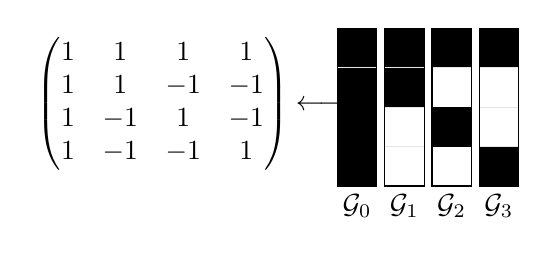
\begin{tikzpicture}[x=0.5cm, y=0.5cm] % {{{
\node at (-2.5,-0.9) {
$
\begin{pmatrix}
1 & 1 & 1 & 1\\
1 & 1 & -1 & -1\\
1 & -1 & 1 & -1\\
1 & -1 & -1 & 1
\end{pmatrix}
\longleftrightarrow
% \mcG_1
$
} ;
\pgfmathsetmacro{\unitstep}{1.2}
% % Coordenadas   {{{
% \node at (-0.6,0.5) {(a)} ;
% \draw[black!10] (0,0) rectangle (1,1); \node at (0.5,0.5) {$\tau_0$} ;
% \begin{scope}[shift={(0,-1)}]
% \draw[black!10] (0,0) rectangle (1,1); \node at (0.5,0.5) {$\tau_1$} ;
% \end{scope}
% \begin{scope}[shift={(0,-2)}]
% \draw[black!10] (0,0) rectangle (1,1); \node at (0.5,0.5) {$\tau_2$} ;
% \end{scope}
% \begin{scope}[shift={(0,-3)}]
% \draw[black!10] (0,0) rectangle (1,1); \node at (0.5,0.5) {$\tau_3$} ;
% \end{scope} 
% \draw (0,-3) rectangle (1,1); 
% % }}}
\begin{scope}[shift={(1*\unitstep,0)}] % Identity {{{
% \begin{scope}[shift={(\unitstep*2,0)}]
\node at (0.5,-3.5) {$\mcG_0$} ;
% \node at (-0.6,0.5) {(b)} ;
\fill[black] (0,0) rectangle (1,1);
\draw[black!10] (0,0) rectangle (1,1);
\begin{scope}[shift={(0,-1)}] \draw[black!10] (0,0) rectangle (1,1); \end{scope}
\begin{scope}[shift={(0,-2)}] \draw[black!10] (0,0) rectangle (1,1); \end{scope}
\begin{scope}[shift={(0,-3)}] \draw[black!10] (0,0) rectangle (1,1); \end{scope}
\draw (0,-3) rectangle (1,1); 
\begin{scope}[shift={(0,-1)}] \fill[black] (0,0) rectangle (1,1); \end{scope}
\begin{scope}[shift={(0,-2)}] \fill[black] (0,0) rectangle (1,1); \end{scope}
\begin{scope}[shift={(0,-3)}] \fill[black] (0,0) rectangle (1,1); \end{scope}
\end{scope} % }}}
\begin{scope}[shift={(2*\unitstep,0)}] % Dephasing {{{
\node at (0.5,-3.5) {$\mcG_1$} ;
\fill[black] (0,0) rectangle (1,1);
% \draw (0,0) rectangle (1,1);
\draw[black!10] (0,0) rectangle (1,1);
\begin{scope}[shift={(0,-1)}] \draw[black!10] (0,0) rectangle (1,1); \end{scope}
\begin{scope}[shift={(0,-2)}] \draw[black!10] (0,0) rectangle (1,1); \end{scope}
\begin{scope}[shift={(0,-3)}] \draw[black!10] (0,0) rectangle (1,1); \end{scope}
\draw (0,-3) rectangle (1,1); 
% \begin{scope}[shift={(0,-1)}] \fill[black] (0,0) rectangle (1,1); \end{scope}
% \begin{scope}[shift={(0,-1)}] \draw (0,0) rectangle (1,1); \end{scope}
\begin{scope}[shift={(0,-1)}] \fill[black] (0,0) rectangle (1,1); \end{scope}
% \begin{scope}[shift={(0,-2)}] \draw (0,0) rectangle (1,1); \end{scope}
% \begin{scope}[shift={(0,-3)}] \fill[black] (0,0) rectangle (1,1); \end{scope}
% \begin{scope}[shift={(0,-3)}] \draw (0,0) rectangle (1,1); \end{scope}
\end{scope} % }}}
\begin{scope}[shift={(3*\unitstep,0)}] % Depolarization {{{
\node at (0.5,-3.5) {$\mcG_2$} ;
% \node at (-0.6,0.5) {(d)} ;
\fill[black] (0,0) rectangle (1,1);
% \draw (0,0) rectangle (1,1);
\draw[black!10] (0,0) rectangle (1,1);
\begin{scope}[shift={(0,-1)}] \draw[black!10] (0,0) rectangle (1,1); \end{scope}
\begin{scope}[shift={(0,-2)}] \draw[black!10] (0,0) rectangle (1,1); \end{scope}
\begin{scope}[shift={(0,-3)}] \draw[black!10] (0,0) rectangle (1,1); \end{scope}
\draw (0,-3) rectangle (1,1); 
% \begin{scope}[shift={(0,-1)}] \fill[black] (0,0) rectangle (1,1); \end{scope}
% \begin{scope}[shift={(0,-1)}] \draw (0,0) rectangle (1,1); \end{scope}
\begin{scope}[shift={(0,-2)}] \fill[black] (0,0) rectangle (1,1); \end{scope}
% \begin{scope}[shift={(0,-2)}] \fill[black] (0,0) rectangle (1,1); \end{scope}
% \begin{scope}[shift={(0,-2)}] \draw (0,0) rectangle (1,1); \end{scope}
% \begin{scope}[shift={(0,-3)}] \fill[black] (0,0) rectangle (1,1); \end{scope}
% \begin{scope}[shift={(0,-3)}] \draw (0,0) rectangle (1,1); \end{scope}
\end{scope} % }}}
\begin{scope}[shift={(4*\unitstep,0)}] % (e) canal malo {{{
\node at (0.5,-3.5) {$\mcG_3$} ;
% \node at (-0.6,0.5) {(e)} ;
\fill[black] (0,0) rectangle (1,1);
% \draw (0,0) rectangle (1,1);
\draw[black!10] (0,0) rectangle (1,1);
\begin{scope}[shift={(0,-1)}] \draw[black!10] (0,0) rectangle (1,1); \end{scope}
\begin{scope}[shift={(0,-2)}] \draw[black!10] (0,0) rectangle (1,1); \end{scope}
\begin{scope}[shift={(0,-3)}] \draw[black!10] (0,0) rectangle (1,1); \end{scope}
% \begin{scope}[shift={(0,-1)}] \fill[black] (0,0) rectangle (1,1); \end{scope}
% \begin{scope}[shift={(0,-1)}] \draw (0,0) rectangle (1,1); \end{scope}
% \begin{scope}[shift={(0,-2)}] \fill[black] (0,0) rectangle (1,1); \end{scope}
% \begin{scope}[shift={(0,-2)}] \draw (0,0) rectangle (1,1); \end{scope}
\begin{scope}[shift={(0,-3)}] \fill[black] (0,0) rectangle (1,1); \end{scope}
% \begin{scope}[shift={(0,-3)}] \draw (0,0) rectangle (1,1); \end{scope}
\draw (0,-3) rectangle (1,1); 
\end{scope} % }}}
\end{tikzpicture} % }}}
\end{document}
